\documentclass{report}
\usepackage{cours}

\linespread{1.2}

\title{Optimization of simplified calculation methods for early age cracking assessment}
\author{Edgar Pierre BURKHART}
\date{2020}

\bibliography{bib}

\begin{document}

\maketitle

\tableofcontents
%%%


\chapter{Literrature review}

\section{Introduction}

Cracking control is a critical point in the design of concrete structures.
Uncontrolled cracking can have a major impact on the durability of reinforced
concrete structures, for several reasons including corrosion of metal rods.
For this reason, the risks of cracking during the early age of a structure have
been studied by numerous research teams in the past. In this chapter, the
results that have been found regarding the evaluation of cracking risks will be
observed.

\section[Creep, Shrinkage and Cracking of Restrained Concrete at Early Age]
{Creep, Shrinkage and Cracking of Restrained Concrete at Early Age
\cite{cscea}}
\subsection{Introduction}
In 2001, a research team from the University of Illinois realised an
experimental study of the impact of creep and shrinkage on cracking of
restrained concrete regarding various parameters.

\subsection{Methods}
An experimental study was conducted using a uniaxial restrained shrinkage test.
A combination of restrained and unrestrained specimens was used to extract
creep from the results. According to the authors, the difference in strain
between free shrinkage and restrained tests was the creep strain, as seen in
\autoref{aci1}. The experiment's goal was to determine a number of properties
of concrete at early age.

This study was conducted with both normal and high performance concrete as
well as plain and fiber reinforced concrete. The aggregates used were always
the same, and both steel fibers and polypropylene fibers were used in fiber
reinforced concrete. The impact of water to cement ratio was studied, at
static temperature and humidity values, with two different drying environements
being used.

\begin{figure}
  \centering
  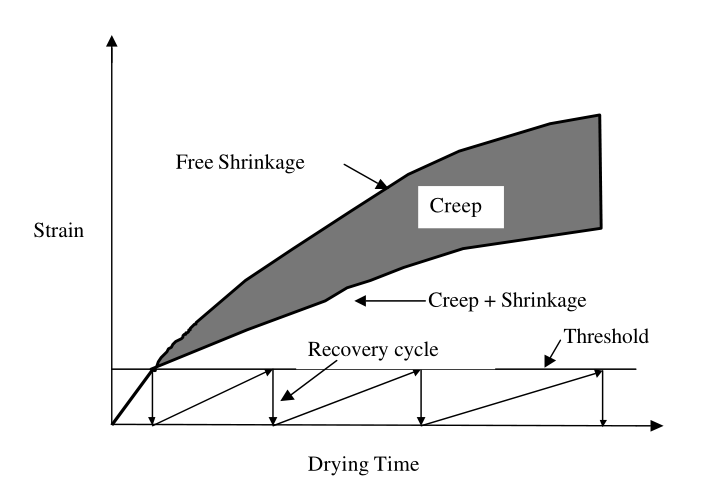
\includegraphics[width=.5\linewidth]{fig/aci1}
  \caption{Schematic diagram of the test mechanism \cite{cscea}.}\label{aci1}
\end{figure}

\subsection{Results}
According to the free shrinkage study, a first stage in which no shrinkage is
experienced by the concrete seems to occur, which is supposed to be caused by
evaporative cooling of the concrete specimens leading to a slight expansion of
the specimens. In the first 10 hours of the study, expansion or shrinkage could
occur depending on the sample.

The results also display a high shrinkage rate during the following 40 hours of
testing. The study of fiber-reinforced concrete showed that steel fibers did
not impact shrinkage, while the use of polypropylene fibers led to a small
increase of free shrinkage.

Although all restrained shrinkage specimens cracked, fracturing time varied
strongly among the different specimens. A lower rate of shrinage was observed
for higher water to cement ratio, causing longer fracturing times. Steel
fiber reinforced specimens also showed delayed fracturing for all water to
concrete ratios, with more higher delays for low water to cement ratios. By
contrast, polypropylene fibers caused earlier failure due to the shrinkage
behavior observed before.

According to the findings of this study, other factors than tensile stress have
an importance in cracking behavior of restrained concrete. For instance,
high-performance concrete cracked earlier than normal concrete despite
sustaining the same tensile stress. Stress history has a strong influence on
the performance of the material regarding cracking. Other findings include that
the failing stress is not equal to the tensile strength of the material, and is
lower by around \SIrange{20}{25}{\percent}.

Relative humidity of the drying environment had an effect on the failing
stress, with lower relative humidities leading to earlier failures, but only
with normal concrete samples.

Creep also had a major impact on cracking by doubling the shrinkage capacity of
a given concrete element. The results highlight a creep to shrinkage ratio of
around \SI{50}{\percent}, with a rapid evolution during the first 2 days
stabiliwing between \num{0.5} and \num{.6}. Fiber reinforcement had little
impact on the creep to shrinkage ratio.

An alternate drying/wetting experiment was also conducted and showed that the
wetting of the concrete led to a high shrinkage recovery rate. An important
note is that the shrinkage rate after a second drying was lower than after the
first continuous drying period. However, creep was also partly reduced by this
approach, and further investigation would be needed to fully understand the
effects of alternate drying and wetting of concrete elements.

\subsection{Conclusion}
The extensive experimental testing conducted for this research paper shows that
several components play a role in the forming of cracks in concrete at
early-age. The study highlights the crucial role of stress rate and history on
the cracking stress and time. It also displays the importance of the actual
tensile strength, which is found to be lower than the usual static tensile
strength. Creep also has a major impact, and should be considered in cracking
studies. Curing practices also seem to have a notable impact on cracking.

\section[State-of-the-Art Report on Control of Cracking in Early Age Concrete]
{State-of-the-Art Report on Control of Cracking in Early Age Concrete \cite{soa}}

\subsection{Introduction}
In 2003, a team of researchers wrote a state-of-the-art on cracking control in
concrete. The goal was to review research on the causes of cracking as well as
the methods that are used to control cracking of concrete.

\subsection{Causes of cracking}
According to this paper, three types of deformation are considered when
studying cracking. Autogenous shrinkage the volume reduction
caused by the hydration of cement in early-age concrete. Drying shrinkage is
created by the evaporation of the water present in early-age concrete. Finally,
thermal shrinkage represents the deformation caused by the changes in concrete
temperature during curing.

These deformation types have a different impact depending on the concrete type.
Low water to cement ratio concretes are more subjected to autogenous shrinkage, while
ordinary concretes tend to be more prone to drying shrinkage.

An important difference between autogenous and drying shrinkage is also the
fact that autogenous shrinkage tends to be uniform in a concrete element, while
drying shrinkage appears more prominently on the surface, leadin to non-uniform
deformations.

Creep also plays a role in cracking by allowing a gradual relaxation of
stresses. The total strain would then be defined by \autoref{eq:1}:
\begin{equation}
  \epsilon_{\text T}(t) =
  \epsilon_{\text{elastic}}(t) +
  \epsilon_{\text{creep}}(t) +
  \epsilon_{\text{shrinkage}}(t) +
  \epsilon_{\text{thermal}}(t)
  \label{eq:1}
\end{equation}

In absence of external loading, this shows that cracking of early-age concrete
is caused by the presence of restraints on deformations of concrete elements.

%%%
\printbibliography
\end{document}
